\documentclass[12pt]{article}
\parindent0em
\parskip 1ex plus 0.4ex minus 0.4ex

\usepackage[a4paper,vmargin=30mm,hmargin=25mm]{geometry}
\usepackage{polyglossia}
\setdefaultlanguage{german}
\usepackage{caption}
\usepackage{fontspec}
\usepackage{lipsum}
\usepackage{xcolor}
\usepackage{listings}
\usepackage{amssymb}
\usepackage{hyperref}
\usepackage{graphicx}
\usepackage{mathtools}
\usepackage{amsfonts}
\usepackage{float}

\definecolor{lstbackground}{rgb}{0.95,0.95,1}      % hellgruener Rahmen
\lstset{language=C}

\lstset{
  basicstyle=\small\ttfamily,
  backgroundcolor=\color{lstbackground},
  keywordstyle=\bfseries\ttfamily\color{blue},
  stringstyle=\color{orange!50!black}\ttfamily,
  commentstyle=\color{gray}\ttfamily,
  showstringspaces=false,
  flexiblecolumns=false,
  tabsize=4,
  numbers=left,
  numberstyle=\tiny,
  numberblanklines=true,
  stepnumber=1,
  numbersep=10pt,
  xleftmargin=15pt,
  literate=%
  {Ö}{{\"O}}1
  {Ä}{{\"A}}1
  {Ü}{{\"U}}1
  {ß}{{\ss}}1
  {ü}{{\"u}}1
  {ä}{{\"a}}1
  {ö}{{\"o}}1
  {~}{{\textasciitilde}}1
}

\begin{document}

\begin{center}
  \textbf{\LARGE Sichere Programmierung} \\[1ex]%
  \textbf{\Large Projekt 2}\\[2ex] %
  Julian Sobott \\ %
  (76511) \\ %
  David Sugar \\ %
  (76050) \\ %
  
\end{center}

\newpage
\tableofcontents
\newpage

% ****************************************************************************
\section{Einleitung}
% ****************************************************************************
Programmiersprachen bzw. Programme zu verstehen geht weit über eine Kenntnis der Syntax und Konventionen hinaus. Hinter jedem Programm, ob Kernel, Dämon oder Nutzer-Programm, versteckt sich eine Abfolge von Maschineninstruktionen, die von ihrem Aufbau kaum noch Ähnlichkeit mit der High-Level-Programmiersprache haben, mit der das jeweilige Programm geschrieben wurde. Dieses tiefere Verständniss zu erlangen, war Zierl dieses Praktikums.



% ****************************************************************************
\section{Zu Aufgabe 1: C-for-Schleifen in Assembler}
% ****************************************************************************
\subsection{a) Analyse des C-Codes}

\textit{gdb-uebung-1.c}

\lstinputlisting{../gdb-uebung-1.c}

Zu beginn der \texttt{main()} Funktion wird eine \texttt{unsigned int} Variable, i, deklariert, jedoch nicht initialisiert, d.h. bis auf wenige Ausnahmen $i \in \{0..2^{32}-1\}$.

Danach wird die Variable im Kopf der darauf folgenden For-Schleife mit 0 initialisiert. Die Schleife inkrementiert die Variable i am Ende jedes Schleifendurchlaufs und tritt erneut in die Schleife ein, solange i kleiner 20 ist.
Innerhalb der Schleife wird der Wert von i, zum jeweiligen Zeitpunkt, formatiert mithilfe von \texttt{printf()} in der Standardausgabe ausgegeben. Dabei werden immer 2 Stellen ausgegeben, dies wird über \texttt{"\%2d"} realisiert.

\textbf{Potentielles Problem: Es sollte \texttt{"\%2u"} verwendet werden, da \texttt{d} für die Formatierung von signed Integern verwendet wird.} In diesem Fall spielt die Formatierung aber keine Rolle.

\subsection{b) Ausführen des Programms}
Das Programm wurde compiliert und ausgeführt. Wie erwartet werden die Zahlen von 0 bis 19 ausgegeben.

\begin{center}
   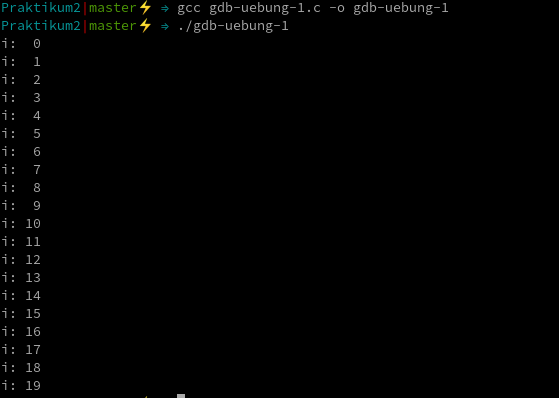
\includegraphics[scale=0.9]{Pictures/aufgabe1b.png}
	\captionof{figure}{Ausgabe von gdb-uebung-1.c}
\end{center}


\subsection{c) Analyse des Assember-Codes}
\begin{lstlisting}
	<+8>:	mov    DWORD PTR [rbp-0x4],0x0
    <+15>:	jmp    0x40113b <main+41>
    <+17>:	mov    eax,DWORD PTR [rbp-0x4]
    <+20>:	mov    esi,eax
    <+22>:	mov    edi,0x402004
    <+27>:	mov    eax,0x0
    <+32>:	call   0x401030 <printf@plt>
    <+37>:	add    DWORD PTR [rbp-0x4],0x1
    <+41>:	cmp    DWORD PTR [rbp-0x4],0x13
    <+45>:	jbe    0x401123 <main+17>
\end{lstlisting}

Für die Variable i wird Speicher auf dem Stack alloziert, die Anfangsadresse ist dabei \texttt{rbp-0x4}.

In Zeile <+8> wird i mit 0x0 initialisiert. Danach springt das Programm unbedingt in Zeile <+41>. Hier befindet sich nun die Überprüfung, ob die Schleife verlassen wird, d.h. $ i \ge 0x14 $, oder ein weiterer Schleifendurchlauf gestartet wird. Dazu wird in Zeile <+41> i mit 0x13 verglichen. Ist der Wert kleiner oder gleich 0x13 wird in Zeile <+17> gesprungen und damit ein weiterer Schleifendurchlauf gestartet. Andernfalls wird die nächste Instruktion ausgeführt und damit die Schleife verlassen.

In Zeile <+17> und <+20> wird der Wert von i, vom Speicher in das \texttt{esi} Register geladen. In der darauf folgenden Zeile wird die Adresse des Formatierungsstrings ("i: \%2d\\n") ( 0x402004 ) in \texttt{edi} geladen.

\begin{lstlisting}
gef➤  x/s 0x402004
0x402004:	"i: %2d\n"
\end{lstlisting}

Weiterhin wird \texttt{eax} wieder auf 0x0 zurückgesetzt. Danach wird \texttt{printf()} mit den in \texttt{edi} und \texttt{esi} geladenen Parametern aufgerufen. Schlussendlich wird i inkrementiert und daraufhin wieder verglichen (<+41>).

\subsection{d) Ausführen des Programms in gdb}

\newcommand{\imageseriesExcercise}[3]{
\begin{center}
   \includegraphics[width=\textwidth]{Pictures/a#1#2_#3.png}
	\captionof{figure}{#3. Ausgabe von gdb-uebung-#1.c}
\end{center}
}


In dieser Aufgabe geht es nun darum das Programm \texttt{gdb-uebung-1.c} in gdb auszuführen. Im folgenden wird der Ablauf durch Screenshots und entsprechende Erklärungen beschrieben.

\imageseriesExcercise{1}{d}{1}


1. Hier beginnt die \texttt{main} Funktion. Als erstes wird der \texttt{rsp} Zeiger, welcher auf den Stack zeigt, um \texttt{0x10} verschoben, um entprechen Platz auf den Stack zu allozieren.

\imageseriesExcercise{1}{d}{2}

2. Initialisieren der Variable i  mit 0x0.

\imageseriesExcercise{1}{d}{3}

3. Unbedingter Sprung in Zeile <main+41>.

\imageseriesExcercise{1}{d}{4}

4. Ausgabe von i. (Adresse: Wert). Der Wert wird in Dezimal ausgegeben.

Schritte bis zur nächsten Zeile wurden übersprungen, da sie in Aufgabe 1 b) ausführlich erklärt wurden.

\imageseriesExcercise{1}{d}{5}

5. Der bedinge Sprung \texttt{jbe} (jump below or equal) wird genommen, da $ 0x0 \le 0x13$. Das heißt, das Programm spring zu <main+17>.

\imageseriesExcercise{1}{d}{6}

6. Schreiben des Wertes von i in eax und eax dann in esi, um i als Parameter an die \texttt{printf} Funktion zu übergeben.

\imageseriesExcercise{1}{d}{7}
\imageseriesExcercise{1}{d}{8}

7.+ 8. Aufrufen der \texttt{printf} Funktion mit i=0. Übergeben wird in rsi und rdi der Wert von i und ein pointer auf den format string. Dieser Aufruf führt zu folgender Ausgabe auf dem Standardoutput:

\begin{lstlisting}
i: 0
\end{lstlisting}

\imageseriesExcercise{1}{d}{9}

9. Hier wird der Wert von i nun um eins erhöht.

\imageseriesExcercise{1}{d}{10}

10. Nach der ausführung ist der Wert 1.

\imageseriesExcercise{1}{d}{11}

11. Als nächstes wollen wir das Programm bis zum letzten Durchlauf laufen lassen und dort dann einen Breakpoint setzen. Als erstes geben wir uns hierfür die Adresse für i aus. Diese wird benötigt, da der Conditional Breakpoint nur stoppen soll, wenn i einen bestimmten Wert hat. In der nächsten Zeile setzen wir den Conditional Breakpoint in die Zeile wo der bedingte Sprung ist (<main+45>). Als Bedingung geben wir an, dass der Wert von i gleich 0x13 sein soll. Wie auch in C müssen Adressen jeweils mit dem * dereferenziert werden. Am Ende wird noch kontrolliert ob der breakpoint richtig gesetzt wurde.

\imageseriesExcercise{1}{d}{12}

12. Lassen wir das Programm nun mit continue (c) laufen, sehen wir alle Schleifendurchläufe mit den entsprechenden Ausgaben. Die letzte Ausgabe ist 18 (0x12).

\imageseriesExcercise{1}{d}{13}

13. Der bedingte Sprung wird ein letztes Mal genommen, da der Wert von i gleich 19 (0x13) ist.

\imageseriesExcercise{1}{d}{14}

14. Die Schleife ist eine letztes Mal durchgelaufen wie erwartet und hat noch die 19 ausgegeben. Wenn wir nun aber an dem bedingten Sprung angkommen wird dier nicht mehr genommen, da die Bedingung nicht mehr zutrifft (i = 0x14 und somit glit nicht mehr i <= 0x13).

\imageseriesExcercise{1}{d}{15}

15. Anstatt an <main+17> zu springen, wurde zur nächsten Anweisung gesprungen <main+47>. Somit wurde die Schleife verlassen. Hier wird noch die 0 als Rückgabewert gespeichert. 

\imageseriesExcercise{1}{d}{16}

16. Mit continue (c) lassen wir das Programm zuende durchlaufen und es wird normal beendet.


% ****************************************************************************
\section{Zu Aufgabe 2: Stackframes}
% ****************************************************************************
\subsection{a) Anlyse des C-Codes}

\textit{gdb-uebung-2.c}

\lstinputlisting{../gdb-uebung-2.c}

Das Programm besteht aus drei Hilfsfunktionen \texttt{f}, \texttt{g}, \texttt{h}, die jeweils 2 int's als Eingabe bekommen und mit Grundrechenarten ein Ergebnis berechnen und zurück geben. Die Berechnungen scheinen willkürlich sein. 

In der \texttt{main} Funcktion, werden zuerst drei int's \texttt{a, b, c} initialisiert werden. Daraufhin wird in einem geschachtelten Funktionsaufruf der Wert von \texttt{c} berechnet. In den Funktionsaufrufen, werden die Rückgabewerte einer Hilfsfunktion immer direkt an die nächste Funktion, als Parameter, übergeben. Am Ende wird durch ein Aufruf der \texttt{printf} Funktion ein formatierter String mit den Werten von den Variablen ausgegeben.


\subsection{b) Ausführen des Programms}

Bild \ref{fig:aufgabe2b} zeigt die Ausgabe des Programms.
\begin{figure}[h!]
	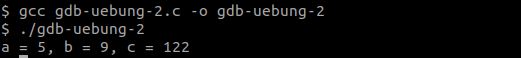
\includegraphics[width=\textwidth]{Pictures/a2b.png}
	\caption{Ausgabe von gdb-uebung-2.c}
	\label{fig:aufgabe2b}
\end{figure}


Wie erwartet sind die Werte von \texttt{a, b} unverändert zur ursprünglichen Initialisierung. Nur \texttt{c} hat den den neuen Wert, den es zugewiesen bekommen hat.

\subsection{c) Stackframes}

\subsubsection{Reihenfolge der Funktionsaufrufe}

Als erstes soll festgestell werde, in welcher Reihenfolge die Funktionen aufgerufen werden. Hierfür wurde in gdb mit s immer der nächste Schritt ausgeführt. Um C-Code zu sehen wurde das Programm mit Debug Informationen compiliert (Option -g bei gcc).

Hier nochmal die relevante Code Zeile:
\begin{lstlisting}
c = f(g(a,h(a,b)),h(b,a));
\end{lstlisting}


\begin{enumerate}
\item \texttt{h(9, 5)} (2. h)
\item \texttt{h(5, 9)} (1. h)
\item \texttt{g(5, 314)}
\item \texttt{f(-692, 314)}
\end{enumerate}

Interessant bei der Ausführung ist, dass bei dem Aufruf von \texttt{f} zuerst der 2. Parameter (\texttt{h} )ausgewertet wird und dann erst der 1. (\texttt{g}).

\subsubsection{Analyse der Stackframes}


Im Folgenden werden die einzelnen Stackframes nun genauer betrachtet. Jedes Stackframe wurde in einem Bild dargestellt. Die Vorlage für so ein Stackframe sieht wie folgt aus. 

\imageseriesExcercise{2}{c}{11}

Hier ist links ein Auschnitt des \textit{Stacks} zu sehen und auf der rechten Seite ein Ausschnitt der \textit{Register}. 

\textbf{Stack}: \newline
Bei dem Stack Ausschnitt ist der relevante Teil in dem sich der StackFrame befindet. Auf der linken Seite vom Stack sind die einzelnen Adressen relativ zum \texttt{RBP} Register angegeben und auf der rechten Seite die Bedeutung des Inhalts. 

Als oberstes steht die \textit{Rücksprungadresse} zu dieser wird zurück gesprungen, wenn die Funktion fertig ausgeführt wird. An dieser Stelle steht immer die Anweisung, die nach dem Aufruf der Funktion kommt. 

Danach kommt der Inhalt des \texttt{RBP} Registers. %TODO Wofür genau!
Als voletztes kommen noch optional lokale Variablen.
Als unterstes im Stack kommt die \texttt{RedZone}, in die nicht geschrieben werden darf.

\textbf{Register}: \newline
In die Register werden die Paramter eingetragen, mit denen die Funktion aufgerufen wurde. Der erste Parameter wird in \texttt{RDI}, der zweite in \texttt{RSI} usw. gespeichert. Werden mehr als 6 Parameter übergeben, werden die restlichen Parameter im Stack gespeichert.

Nun kann jeder Inhalt des Stackframes gelesen werden. Pointer im Stack wurden aufgelöst um besser zu sehen wohin z.B. die Rücksprungadresse zeigt. Anonsten würden an den entsprechenden Stellen Adressen stehen. Das Programm wird wieder ausgeführt und am Anfang einer Funktion weren die Daten notiert.

\imageseriesExcercise{2}{c}{0}
Zu sehen ist, dass als Paramter die die aus Paramter übergeben wurden. In unserem Fall nur die Anzahl und der Name des Programms. Führt man die Zeile in der die Variablen initialisiert werden, sieht man auch diese Werte im Stack.

\imageseriesExcercise{2}{c}{1}
Die Funktion \texttt{h} wurde aufgerufen und die entsprechenden Parameter sind in den Registern zu sehen. Außerdem sieht man, dass die Rücksprungadresse nun in eine Zeile in der \texttt{main} Funktion zeigt und nicht wie zuvor in C internen Code.

\imageseriesExcercise{2}{c}{2}
Zweiter Aufruf der Funktion \texttt{h} mit umgedrehten Paramtern un höherer Rücksprungadresse. 

\imageseriesExcercise{2}{c}{3}
Aufruf der Funktion \texttt{g} mit dem Wert aus der Variable \texttt{a} und dem Rückgabewert der Funktion \texttt{h}.

\imageseriesExcercise{2}{c}{4}
Aufruf der Funktion \texttt{f} mit den Rückgabewerten der Funktionen \texttt{g, h}.








\newpage
% ****************************************************************************
\section{Zu Aufgabe 3}
% ****************************************************************************
\subsection{a) Analysieren Sie den in der Datei enthaltenen Source Code}
Das bereitgestellte Quelldatei \texttt{gdb-uebung-3.c} enthält die rekursive Implementierung eines \textbf{Factorial-Algorithmus}, damit ist $f(n) = n! $.

\textbf{Def:} $ n! = n * (n-1) * (n-2) * ... * 1 = \prod_{i = 1}^{n} i ,\;  n \in \mathbb{N} $

\subsubsection{Implementierung}
\begin{figure}[h]
\begin{lstlisting}
unsigned int f(unsigned int i) {
  if (i>1) {
    return i * f(i-1);
  } else {
    return 1;
  }
}
\end{lstlisting}
\label{fig:factorial}
\caption{factorial function}
\end{figure}

Die Funktion, abgebildet in \ref{fig:factorial} nimmt einen vorzeichenlosen Integer als Argument und gibt als Ergebnis ebenfalls einen vorzeichenlosen Integer zurück. Dabei ist \textbf{int} jedoch betriebssystemabhängig definiert. Für die meisten Systeme kann jedoch angenommen werden, dass es sich dabei um ein \textbf{4 Byte} großes Wort handelt, d.h für den Rückgabewert kommen Werte innerhalb des Wertebereichs $  W = [0,2^{32}-1] $ in Frage. Aufgrund des extrem schnellen Wachstums von $ n! $ ist dies ein sehr beschränkender Faktor, der bei der Nutzung unbedingt mit zu berücksichtigen ist, da es schnell zu einem Überlauf und damit zu einer Verfälschung des Ergebnisses kommen kann. In Zeile 2 wird danach geprüft, ob der übergebene Wert größer 1 ist. Sollte dies der Fall sein, wird das  Produkt von i und dem Ergebnis des Rekursiven Aufrufs von $ f(i-1) $ zurückgegeben. Andernfalls wird die Konstante 1 als Rückgabewert der Funktion genutzt, siehe Zeile 5.
\newpage

\subsubsection{Aufruf}
\begin{figure}[h]
\begin{lstlisting}
int main() {
  unsigned int i=5, r=0;

  r = f(i);

  printf("i = %d, f(i) = %d\n", i, r);
}
\end{lstlisting}
\label{fig:factorial-main}
\caption{invocation of f()}
\end{figure}

In der \textbf{main()} Funktion wird die in \ref{fig:factorial} beschriebene Funktion \textbf{f(unsigned int)} aufgerufen und dabei \textbf{i = 5} als Argument übergeben. Das Ergebnis des Aufrufs wird der Variable \textbf{int r} zugewiesen, siehe Zeile 4. Danach wird \textbf{i} und das Ergebnis \textbf{r} mittels \textbf{printf()} auf der Kommandozeile ausgegeben.

\subsection{b) Kompilieren Sie den C Code und führen Sie das Programm aus }
\subsubsection{Kompilieren}
Das Kompilieren des Quellkodes innerhalb von \texttt{gdb-uebung-3.c} kann mittels des folgenden Befehls auf der Kommandozeile ausgeführt werden.
\begin{lstlisting}
$ gcc gdb-uebung-3.c -o gdb-uebung-3
\end{lstlisting}
Der in diesem Fall genutzte Compiler heißt \textbf{gcc} (GNU compiler collection). Dabei ist gdb-uebung-3.c der Name der Quelldatei. Mittels \textbf{-o gdb-uebung-3} wird der gewünschte Name, der zu erstellenden Programmdatei, angegeben.

\subsubsection{Ausführen}
Das Programm kann nun auf der Kommandozeile ausgeführt werden.
\begin{lstlisting}
$ ./gdb-uebung-3                    
i = 5, f(i) = 120
\end{lstlisting}
Zum verifizieren des Ergebnisses kann dieses auch noch einmal Händisch berechnet werden, $ \prod_{i = 1}^{5} i = 1 * 2 * 3 * 4 * 5 = 2 * 3 * 20 = 2 * 60 = 120 $. Das Ergebnis stimmt, die Funktionen scheint auf den ersten Blick also richtig implementiert. Um nachzuvollziehen, wie die das Ergebnis zustande kommt, kann der folgende Graph betrachtet werden.

\begin{center}
\begin{figure}[h]
	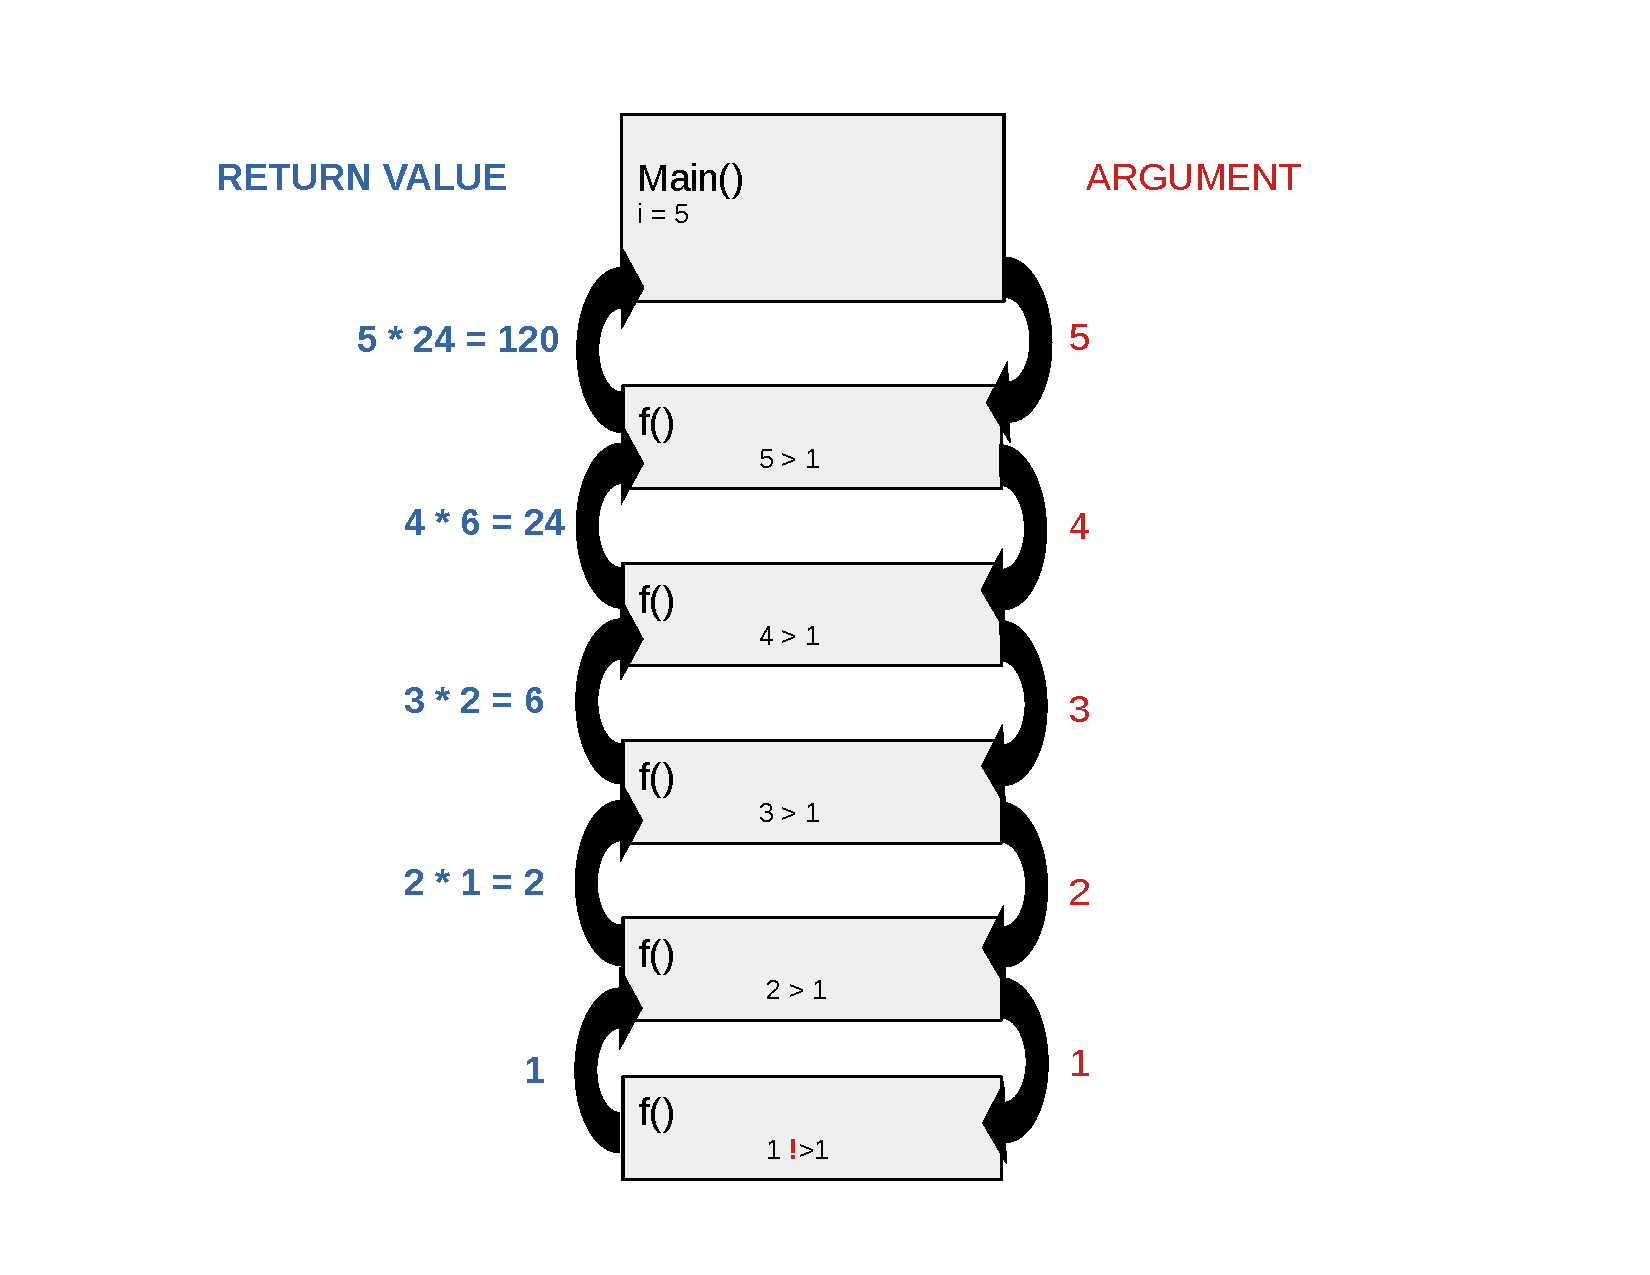
\includegraphics[scale=0.6]{Pictures/aufgabe3aufrufe.pdf}
	\caption{recursive call of f()}
	\label{fig:recursive2}
\end{figure}
\end{center}

Anfangs wird in \textbf{main()} die Funktion \textbf{f()} mit \textbf{5 als Argument} aufgerufen. Die aufgerufene Funktion f(5) prüft nun, ob der Parameter größer als 1, d.h. \textbf{5 > 1}, ist. Ist dies der Fall, ruft sich die Funktion selbst wieder auf, dieses Mal jedoch mit dem \textbf{dekrementierten} Parameter als Argument. Dies wiederholt sich bis 1 bzw. 0 übergeben wird, in diesem Fall wird 1 zurückgegeben und das Ergebnis 'aufsteigend' berechnet.

\subsection{c) Führen Sie das Programm im GDB aus}




\subsubsection{Wie viele Stack Frames werden erzeugt?}
Um die Anzahl der \textbf{Stack Frames} in GDB zu ermitteln, kann man wie folgt vorgehen.
\begin{itemize}
	\item Wir wissen:
	\begin{itemize}
		\item Das Programm ruft sich selber rekursiv auf.
		\item Dies geschieht solange der übergebene Parameter > 1 ist.
		\item Andernfalls wird 1 zurückgegeben.
		\item Der Parameter wird innerhalb von f() dekrementiert und als Argument wieder an f() übergeben.
		\item Das Argument wird bei jedem rekursiven Aufruf wird mittels \textbf{RDI} übergeben (siehe \ref{sec:calling_convention}).
	\end{itemize}
\end{itemize}

D.h. wenn ein Bedingter Break Point so gesetzt wird, dass das Programm am Anfang der aufgerufenen Funktion f() anhält, genau dann wenn \textbf{RDI = 1} ist, können wir bequem die Anzahl der Stack Frames ablesen. Denn in diesem Fall können wir sicher sein, dass kein weiteres Mal f() rekursiv aufgerufen wird.

\begin{lstlisting}
gef>  break f if $rdi == 1
gef>  r
\end{lstlisting}

Das Programm wird nun bei maximaler Tiefe \textbf{t = 6}, der Funktionsaufrufe angehalten. Diese Tiefe entspricht auch der Anzahl der Stack Frames, da für jeden Funktionsaufruf ein eigener Frame angelegt wird.

\imageseriesExcercise{3}{c}{1}

\subsubsection{Wie ist der Inhalt dieser Stack Frames?}
Die Werte der Rücksprungadressen, Frame und Stack Pointer sind aufgrund von \textbf{Address Space Layout Randomisation (ASLR)} immer unterschiedlich (bis auf die letzten 12 Bit), deshalb werden im Anschluss relative Adressen angegeben.

Main als auch f() allozieren für sich jedes mal 16 Byte auf dem Stack. 
\begin{lstlisting}
MOV rbp, rsp
SUB rsp, 0x10	// allocate 16 bytes on the heap
\end{lstlisting}

f() speichert dann den übergebenen Wert direkt unter dem gespeicherten Frame Pointer. Am Schluss wird das berechnete Ergebnis in main(), auf den Stack an Stelle rbp-0x8 geschrieben (rote Markierung \ref{fig:recursive3} in main).

\begin{center}
\begin{figure}[H]
	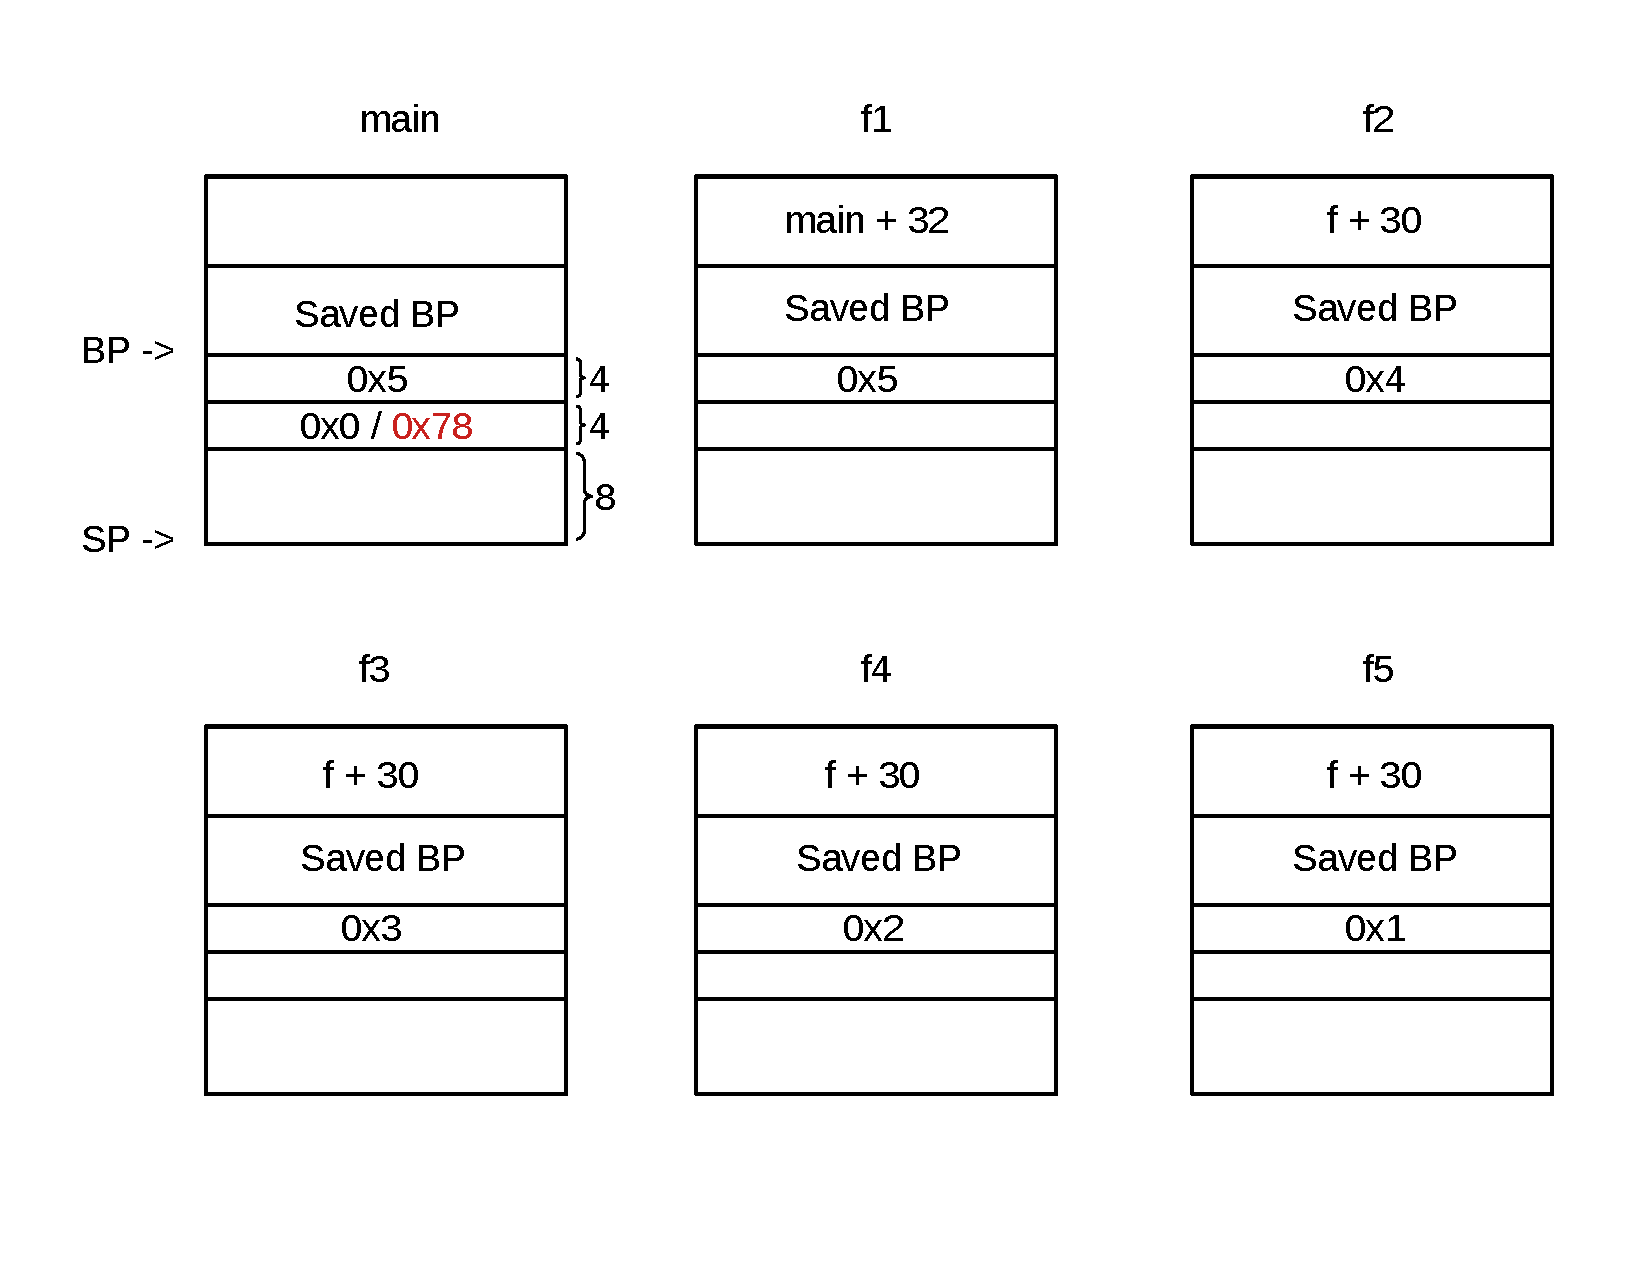
\includegraphics[scale=0.8, angle=90]{Pictures/a3_stack_frames.pdf}
	\caption{Stack Frames aller Funktionsaufrufe für i = 5}
	\label{fig:recursive3}
\end{figure}
\end{center}



\subsubsection{Wie wird die Parameterübergabe in Assembler umgesetzt?}
\label{sec:calling_convention}
Für die Übergabe von Parametern an Subroutinen muss unter x86 eine Fallunterscheidung gemacht werden. Je nachdem, ob es sich um Programme für ältere 32-Bit Prozessoren handelt oder um Programme für neuere 64-Bit Prozessoren, werden verschiedene sog. \textbf{Calling Conventions} (Aufruf Konventionen) verwendet. Diese Konventionen dienen dazu einen Ablauf zu definieren, sodass unabhängig vom Autor des Codes darauf vertraut werden kann, dass Abläufe wie z.B. ein Unterprogrammaufruf \textbf{immer} auf die selbe Weise durchgeführt werden.

\subsubsection*{32-Bit}
Ein Unterprogrammaufruf kann in folgende Schritte untergliedert werden.
\begin{enumerate}
\item Zuerst müssen die \textbf{Caller Saved Register}, falls nötig, auf dem Stack gespeichert werden, da die \textbf{aufgerufene} Funktion für diese Register keine Garantie übernimmt, dass diese nicht überschrieben werden. Die Register sind: ebx, ecx, edx, r10, r11.

\item Danach müssen die Parameter in \textbf{umgekehrter Reihenfolge} auf den Stack gepushed werden. Aufgrund der Funktionsweise des Stacks ist dann der Erste Parameter der Subroutine direkt angrenzend and die gespeicherte Rücksprungadresse, die im nächsten Schritt auf dem Stack hinterlegt wird.

\item Nun wird mit \textbf{call} der Unterprogrammaufruf durchgeführt. Dabei wird die \textbf{Rücksprungadresse} (die Adresse des auf call folgenden Befehlswortes) auf den Stack gepushed und ein Sprung zum ersten Befehl des Unterprogramms, markiert durch das angegebene \textbf{Label}, gesprungen.

\item Die ersten Befehle des Unterprogramms bilden einen sog. \textbf{Function Prologue}. Hier werden als aller erstes die Werte der \textbf{Callee Save Register}, falls die entsprechenden Register benötigt werden, sowie der \textbf{Base Pointer (bp)} auf den Stack gepushed. Danach wird der Aktuelle Wert des \textbf{Stack-Pointers (sp)} genutzt um den für den derzeitigen \textbf{Stack-Frame} verantwortlichen bp zu initialisieren, indem der Wert von sp in bp verschoben wird. Danach wird der sp mit \textbf{SUB} verringert um Speicher auf dem Stack für lokale Variablen zu allozieren.

\item Am Ende der Subroutine wird dann der sog. \textbf{Function Epilogue} ausgeführt. Als erstes wird der Wert von bp wieder in sp verschoben, wodurch der allozierte Speicherplatz auf dem Stack wieder freigegeben wird. Danach werden die im Epilogue gepushten Werte, in sinngemäß umgekehrter Reihenfolge in die jeweiligen Register gepoppt. Der Rückgabewert wird in das \textbf{A-Register} verschoben und schlussendlich mit dem \textbf{RET} Befehl das Unterprogramm wieder verlassen, indem zur gespeicherten Rücksprungadresse gesprungen wird.  
\end{enumerate}

\newpage
\subsubsection*{64-Bit}
Ein Unterprogrammaufruf unter 64-Bit läuft wie oben beschrieben ab, mit einer Änderung. Die Argumente werden hier mithilfe von Registern übergeben. Das erste Argument wird über \textbf{RDI} und die weiteren mithilfe von \textbf{RSI}, \textbf{RDX}, \textbf{RCX}, \textbf{r8}, \textbf{r9} übergeben. Sollten mehr Argumente übergeben werden müssen, dann werden diese wie oben beschrieben mittels Stack übergeben.

\begin{figure}[H]
\begin{lstlisting}
// #### PROLOGUE ####
PUSH	rbp			// save rbp on the stack
MOV		rbp, rsp
SUB		rsp, 0x10	// allocate 16 byte on the stack

...

// #### EPILOGUE ####
MOV		rsp, rbp	// deallocate memory
POP		rbp			// restore old base pointer
RET					// return to calling function
\end{lstlisting}
\label{lst:epipro}
\caption{Typischer Funktionsprolog und -epilog}
\end{figure}

\subsubsection*{Programmbeispiel}
Ein Beispiel für einen Funktionsaufruf mit Argumentübergabe ist folgende Stelle.
\imageseriesExcercise{3}{c}{0}
Hier wird, bevor f() aufgerufen wird, der Wert von i (5), welcher sich in EAX befindet mittels MOV nach EDI verschoben. In f() selber wird dann als erstes Platz für lokale Variablen und Parameter geschaffen, indem Speicher alloziert wird.
\imageseriesExcercise{3}{c}{2}
Danach wird das übergebene Argument von EDI, für die weitere Nutzung, nach rbp-0x4 verschoben. Dies spiegelt einen typischen 64-Bit Funktionaufruf unter x86 wieder. 

\newpage
% ****************************************************************************
\section{Zu Aufgabe 4}
% ****************************************************************************
\subsection{a) Analysieren Sie den in der Datei enthaltenen Source Code}
\subsubsection{Analyse}
Das gegebene Programm soll die Summe mehrere Fließkommazahlen mittels einer Schleife berechnen. Dabei wird ebenfalls ein Float als Laufvariable i in der Schleife verwendet. Die Schleife zählt dabei, in jeder Iteration, zur Summe den aktuellen Wert von i hinzu. Danach wird ein Zähler namens anzahl inkrementiert und zu i der Wert 0.01 hinzugezählt. Die Schleife wird solange ausgeführt, wie i den Wert 1000.03 nicht übersteigt.

\lstinputlisting{../gdb-uebung-4.c}

Am Ende wird dann noch der in Zeile 13 zu sehende, formatierte String ausgegeben. Aufgrund der Benutzung einer Fließkommazahl, ist eine gewisse Ungenauigkeit mit einzurechnen, da Fließkommazahlen nur annäherungsweise in Computern dargestellt werden können.

\subsubsection{Floating Point Numbers}
Grundlegend unterscheidet man in \textbf{32-Bit Floating point Zahlen} (float) und \textbf{64-Bit (double precision) Floating Point Zahlen} (double). Der \textbf{IEEE 754 32-bit floating-point standard} ist z.B. wie folgt definiert.
\imageseriesExcercise{4}{a}{0}
Dabei wird die Zahl intern in drei Teilbereichen dargestellt. \textbf{S} gibt das Vorzeichen an, d.h. 0 bedeutet positiv und 1 negativ. 

Die Zahl selber wird normalisiert abgespeichert, d.h. die Fließkommazahl wird so verschoben, dass nur eine 1 vor dem Komma steht. Damit man die Zahl später wieder rekonstruieren kann, wird der Exponent um den verschoben wurde plus 127 mit abgespeichert. Man spricht dann auch vom \textbf{biased exponent}, da zu ihm ein Bias hinzugefügt wurde. Aufgrund der Tatsache, dass durch diese Normalisierung immer eine einzige 1 vor dem Komma steht, wird diese in der internen Darstellung nicht mit angegeben, dadurch steht ein weiteres Bit für die \textbf{fraction} zur Verfügung. Ein floating point Zahl f kann demnach wie folgt angegeben werden.

\begin{figure}[H]
\begin{center}
\[f = (-1)^{S} * 1.fraction * 2^{E-127}\]
\end{center}
\label{math:ieefp:1}
\caption{IEEE 32-bit floating point}
\end{figure}

\subsubsection*{Beispiel}
\begin{figure}[H]
\begin{center}
\[
-0.125_{10} = -0.001_{2}
= (-1)^{1} * 1.0 * 2^{-3}
= (-1)^{1} * 1.0 * 2^{-3+127-127}
= (-1)^{1} * 1.0 * 2^{124-127}
\]
\end{center}
\label{math:ieefp:2}
\caption{Beispiel anhand von -0.125}
\end{figure}

Daraus ergibt sich:
\begin{table}[H]
\begin{tabular}{l l l}
S & E & fraction \\
1 & 01111100 & 00000000000000000000000\\
\end{tabular}
\end{table}

\subsection{b) Kompilieren Sie den C Code und führen Sie das Programm aus }
\subsubsection{Kompilieren}
Das Kompilieren des Quellkodes innerhalb von \texttt{gdb-uebung-4.c} kann mittels des folgenden Befehls auf der Kommandozeile ausgeführt werden.
\begin{lstlisting}
$ gcc gdb-uebung-4.c -o gdb-uebung-4
\end{lstlisting}
Der in diesem Fall genutzte Compiler heißt \textbf{gcc} (GNU compiler collection). Dabei ist gdb-uebung-3.c der Name der Quelldatei. Mittels \textbf{-o gdb-uebung-3} wird der gewünschte Name, der zu erstellenden Programmdatei, angegeben.

\subsubsection{Ausführen}
Das Programm kann nun auf der Kommandozeile ausgeführt werden.
\begin{lstlisting}
$ ./gdb-uebung-4                    
Summe: 3000.030029, Anzahl: 3
\end{lstlisting}
Das Ergebnis überrascht jedoch zuerst. Eigentlich hätte es zu einem weiteren Durchlaufen der Schleife kommen sollen und auch das Ergebnis weicht um 0.000029 vom erwarteten Zwischenergebnis 3000.03 ab.

Tabellarisiert haben die Variablen zum n'ten Schleifendurchlauf folgende Zustände.
\begin{table}[H]
\begin{tabular}{l | l l l}
n & summe & i & anzahl \\
\hline
0 & 0 & 1000 & 0 \\
1 & 1000.0 & 1000.01 & 1 \\
2 & 2000.01 & 1000.02 & 2 \\
3 & 3000.03 & 1000.03 & 3 \\
4 & \textbf{4000.06} & 1000.04 & 4 \\
\end{tabular}
\end{table}

\subsection{c) Analysieren Sie das Programm mit dem GDB }

\subsubsection{Berechnet die Schleife das korrekte Ergebnis?}
Nein, wie oben beschrieben weicht das Ergebnis von dem erwarteten Ergebnis ab.

\subsubsection{Welche Werte nehmen die Variablen bei der Ausführung des Programms an?}
Das das Programm mit Floatingpoint-Zahlen rechnet gilt es als erstes einige Befehle zu erläutern, die das Programm in diesem Fall nutzt und die nur auf diesem Datentyp operieren.

\subsubsection*{Floating Point Instruktionen}
\begin{description}
	\item [xmm0-15] - Floating Point Register

	\item [movss <dest>, <src>] - Kopiert einen 32-Bit Quell-Operanden in einen 32-Bit Ziel-Operanden.

	\item [movsd <dest>, <src>] - Kopiert einen 64-Bit Quell-Operanden in einen 64-Bit Ziel-Operanden.

	\item [cvtsd2ss <dest>, <src>] - Wandelt einen 64-Bit FP Quell-Operanden in einen 32-Bit FP Zahl um und kopiert sie nach <dest>.

	\item [cvtss2sd <dest>, <src>] - Wandelt einen 32-Bit FP Quell-Operanden in einen 64-Bit FP Zahl um und kopiert sie nach <dest>.

	\item [addss <dest>, <src>] - <32-Bit dest> := <32-Bit dest> + <32-Bit src>

	\item [addsd <dest>, <src>] - <64-Bit dest> := <64-Bit dest> + <32-Bit src>

	\item [ucomisd <RXsrc>, <src>] - Vergleich der beiden 64-Bit FP Register <RXsrc> und <src>. Ein Operand kann auch eine Speicheradresse sein.
\end{description}


\subsubsection*{Analyse}
Um die Werte über die verschiedenen Schleifendurchläufe hinweg verfolgen zu können, muss als ersten ein Breakpoint an den Kopf der Schelife gestzt werden. Dafür gilt es den Kopf der Schleife mittels \textbf{GDB} zu ermittlen.

Da sich der komplette Programmcode in \textbf{main()} befindet, wird diese Funktion auch disassembliert.
\begin{lstlisting}
gef> disass main

   <+0>:	push   rbp
   <+1>:	mov    rbp,rsp
   <+4>:	sub    rsp,0x10
   <+8>:	pxor   xmm0,xmm0
   <+12>:	movss  DWORD PTR [rbp-0x8],xmm0
   <+17>:	mov    DWORD PTR [rbp-0xc],0x0
   <+24>:	movss  xmm0,DWORD PTR [rip+0x116]        # 0x780
   <+32>:	movss  DWORD PTR [rbp-0x4],xmm0
   <+37>:	jmp    0x69e <main+84>
   <+39>:	movss  xmm0,DWORD PTR [rbp-0x8]
   <+44>:	addss  xmm0,DWORD PTR [rbp-0x4]
   <+49>:	movss  DWORD PTR [rbp-0x8],xmm0
   <+54>:	add    DWORD PTR [rbp-0xc],0x1
   <+58>:	cvtss2sd xmm0,DWORD PTR [rbp-0x4]
   <+63>:	movsd  xmm1,QWORD PTR [rip+0xf7]        # 0x788
   <+71>:	addsd  xmm0,xmm1
   <+75>:	cvtsd2ss xmm2,xmm0
   <+79>:	movss  DWORD PTR [rbp-0x4],xmm2
   <+84>:	cvtss2sd xmm0,DWORD PTR [rbp-0x4]
   <+89>:	movsd  xmm1,QWORD PTR [rip+0xe5]        # 0x790
   <+97>:	ucomisd xmm1,xmm0
   <+101>:	jae    0x671 <main+39>
   <+103>:	cvtss2sd xmm0,DWORD PTR [rbp-0x8]
   <+108>:	mov    eax,DWORD PTR [rbp-0xc]
   <+111>:	mov    esi,eax
   <+113>:	lea    rdi,[rip+0xa6]        # 0x768
   <+120>:	mov    eax,0x1
   <+125>:	call   0x520 <printf@plt>
   <+130>:	mov    eax,0x0
   <+135>:	leave
   <+136>:	ret
\end{lstlisting}
Danach muss die Abfolge von Instruktionen, die nun erscheint, auf Instruktionsblöcke hin abgesucht werden, die auf genau so einen Kopf schließen lassen. Gleichzeitig können einzelne Speicheradressen und Register, durch Analyse genau dieser Adressen, den passenden Variablen im Quelltext zugeordnet werden. Dies hilft, den Code besser verstehen und vergleichen zu können.

Bei <main + 12> wird der 32-Bit FP Wert 0 aus Register \textbf{xmm0} an Adress \textbf{rbp-0x8} copiert. Da es nur ein FP Variable im Quelltext gibt, die mit 0 initialisiert wird, fällt die Zuordnung in diesem Fall leicht. Es muss sich bei der Speicheradress rbp-0x8 um die Variable \textbf{summe} handeln.
\begin{lstlisting}
<+12>:	movss  DWORD PTR [rbp-0x8],xmm0		; summe := 0
\end{lstlisting}

Ähnlich verhällt es sich hier mit der darauf folgenden Zeile. Da bis auf eine Ausnahme mit FP Zahlen gerechnet wird, muss es sich bei Instruktion <main + 17> um die Initialisierung der Integer-Variable \textbf{anzahl} mit 0 handeln.
\begin{lstlisting}
<+17>:	mov    DWORD PTR [rbp-0xc],0x0		; anzahl := 0
\end{lstlisting}

Daraufhin wird der Wert an Adresse \textbf{rip+0x116} in xmm0 kopiert und danach gleich wieder an Adresse \textbf{rbp-0x4} geschrieben. Da mit rip+0x116 die Adresse relativ zum Instruktions-Pointer angegeben wird, kann davon ausgegangen werden, dass der Wert in der schreibgeschützten \textbf{Text-Section} befindet. Damit muss es sich hierbei um eine Konstante handeln. Die Konstanten, die in dem gegebenen Programm vorkommen sind \texttt{1000, 1000.03 und 0.01}.
\begin{lstlisting}
<+24>:	movss  xmm0,DWORD PTR [rip+0x116]
<+32>:	movss  DWORD PTR [rbp-0x4],xmm0
\end{lstlisting}
Um den exakten Wert zu erhalten und damit eine Zuordnung vornehmen zu können gilt es die Speicheradresse zu inspizieren. Dabei wird die \textbf{f Option} gewählt, da es sich mit hoher Wahrscheinlichkeit um ein FP Zahl an der zu inspizierenden Adresse handelt.
\begin{lstlisting}
gef> x/f 0x780
0x780:	1000
\end{lstlisting}
Und tatsächlich scheint es sich bei den Instruktionen um die Initialisierung von \textbf{i} mit dem Wert 1000.0 zu handeln.

\textbf{Zuordnung}
\begin{itemize}
	\item anzahl = rbp-0xc	(32-Bit int)
	\item summe  = rbp-0x8	(32-Bit float)
	\item i	     = rbp-0x4	(32-Bit float)
\end{itemize}

Mit dieser Zuordnung ist nun klar, welche Adressen im Speicher (Variablen) es zu beobachten gilt.

Nun gilt es noch den Kopf der Schleif ausfindig zu machen. Die Instruktion an Stelle <main + 37> springt an Adresse <main + 84>. Hier wird als erstes die 32-Bit FP Zahl \textbf{i} in eine 64-Bit FP Zahl umgewandelt und nach xmm0 kopiert. Danach wird die Konstante 1000.03 in xmm1 copiert. xmm0 und xmm1 werden daraufhin verglichen und falls 1000.03>= i ist, wird an die Stelle <main + 39> gesprungen.
\begin{lstlisting}
<+84>:	cvtss2sd xmm0,DWORD PTR [rbp-0x4]	; xmm0 := i
<+89>:	movsd  xmm1,QWORD PTR [rip+0xe5]	; xmm1 := 1000.03
<+97>:	ucomisd xmm1,xmm0			; while 1000.03 >= i:
<+101>:	jae    0x671 <main+39>			;	...
\end{lstlisting}
Damit ist der Kopf der Schleife Gefunden. Nun kann ein Breakpoint an Stelle <main+84>, d.h. Adresse 0x69e gestzt werden. Dazu wird als erstes ein Breakpoint an den Anfang von main() gesetzt und das Programm gestartet.
\begin{lstlisting}
gef> break main
gef> r
\end{lstlisting}
Der Prozess wird nun gleich nach dem Function Prologue \ref{lst:epipro} angehalten. 

\imageseriesExcercise{4}{c}{0}

Mit \textbf{disass main} können nun noch einmal alle Instruktionen angezeigt werden. Diesmal enthällt jede Spalte jedoch zusätzlich noch die jeweilige Adresse im Speicher. Diese können wir nun Nutzen um den Breakpoint an den Schleifenkopf zu setzen. Außerdem wird noch ein Breakpoint hinter die \textbf{jae} Instruktion gesetzt, damit sich das Programm nich sofort, nach dem letzten Schleifendurchlauf beendet. Mit \textbf{continue} wird der Prozess danach bis zum nächsten Breakpoint fortgesetzt.
\begin{lstlisting}
gef> break *0x000055555555469e		; address can differ
gef> break *0x00005555555546b1
gef> c
\end{lstlisting}

\imageseriesExcercise{4}{c}{1}

Um die Werte der einzelnen Variablen abzufragen, kann wieder der \textbf{x} (examine) Befehl verwendet werden. Zum 0'ten Schleifendurchlauf halten die Variablen \textbf{anzahl, summe, i} folgende Werte.

\begin{lstlisting}
gef> x/d $rbp-0xc
0x7fffffffe7d4:	0	; anzahl
gef> x/f $rbp-0x8
0x7fffffffe7d8:	0	; summe
gef> x/f $rbp-0x4
0x7fffffffe7dc:	1000	; i
gef> c
\end{lstlisting}

Nach dem 1'ten Schleifendurchlauf halten die Variablen \textbf{anzahl, summe, i} folgende Werte. Hier fällt bei \textbf{i} auf, dass nicht wie erwartet exakt 0.01 zu i addiert wurde, sondern eine leicht höhere Zahl. D.h. die Addition der FP Zahl 0.01 zu i stellt einen Defekt in dem gegebenen Programm dar. Durch diesen wurde die Variable i infiziert.

\begin{lstlisting}
gef> x/d $rbp-0xc
0x7fffffffe7d4:	1	; anzahl
gef> x/f $rbp-0x8
0x7fffffffe7d8:	1000	; summe
gef> x/f $rbp-0x4
0x7fffffffe7dc:	1000.01001	; i
gef> c
\end{lstlisting}

Nach dem 2'ten Schleifendurchlauf halten die Variablen \textbf{anzahl, summe, i} folgende Werte. Auch hier verschlimmert sich die Infektion, d.h. i weicht noch mehr vom zu erwartenden Wert ab.

\begin{lstlisting}
gef> x/d $rbp-0xc
0x7fffffffe7d4:	2	; anzahl
gef> x/f $rbp-0x8
0x7fffffffe7d8:	2000.01001	; summe
gef> x/f $rbp-0x4
0x7fffffffe7dc:	1000.02002	; i
gef> c
\end{lstlisting}

Nach dem 3'ten Schleifendurchlauf halten die Variablen \textbf{anzahl, summe, i} folgende Werte.

\begin{lstlisting}
gef> x/d $rbp-0xc
0x7fffffffe7d4:	3	; anzahl
gef> x/f $rbp-0x8
0x7fffffffe7d8:	3000.03003	; summe
gef> x/f $rbp-0x4
0x7fffffffe7dc:	1000.03003	; i
gef> c
\end{lstlisting}

Nach dem 3'ten Schleifendurchlauf kommt es zu einem Abbruch der Schleife, da die Bedingung nicht mehr erfüllt ist, d.h. $ i = 1000.03003 \nleq 1000.03 $. Was wiederrum zu dem Fehlverhalten des Programms führt.

\subsubsection{Warum wird das falsche Ergebnis berechnet?}
Computer haben ein großes Problem, wenn es um die Darstellung von Fließkommazahlen geht. Dazu kann man sich folgende Frage Stellen. Man nehme zwei Zahlen, n = 0.0000001 und m = 0.0000002. \textbf{wie viele Zahlen liegen zwischen n und m?}. Die Antwort ist weniger überraschend, nämlich \textbf{unendlich viele}. Dies gilt natürlich für zwei beliebige Reelle Zahlen n und m, zeigt aber das Problem der Endlichkeit von Computern. 

Das Programm nutzt z.B. 32-Bit Floating Point Zahlen. Wenn man vom IEE 754 FP Standard ausgeht, bedeutet das, dass 23 Bit für die Darstellung einer Kommazahl zur verfügung stehen, plus 9-Bit für Exponent und Vorzeichen. Damit können natürlich nicht unendlich viele reelle Zahlen dargestellt werden. Zahlen werden \textbf{näherungsweise} dargestellt, d.h. anstelle der eigentlichen Zahl wird die nächstmögliche Zahl verwendet, die darstellbar ist. Dabei ist die Wertigkeit der einzelnen Stellen zu berücksichtigen.

\subsubsection*{Wertigkeit der Stellen zur Basis 2}
\begin{table}[H]
\begin{tabular}{c c c c c c c}
	... & $ 2^{2}$ & $ 2^{1} $ & $ 2^{0} $ & $ 2^{-1} $ & $ 2^{-2} $ & ... \\
	... & 4 & 2 & 1 & 0.5 & 0.25 & ... \\
\end{tabular}
\end{table}


Um die näherungsweise Darstellung zu illustrieren kann von einem vereinfachten Beispiel mit Festkommazahl ausgegangen werden.

\subsubsection*{Beispiel}
\begin{itemize}
	\item Sei R 8-Bit Register mit 1 Vorkomma- und 7 Nachkommastellen ohne Vorzeichen.
	\item D.h. $ R = V.NNNNNNN $
	\item Speichere 0.1 binär in Register R.
	\item dann ergibt sich die näherungsweise Darstellung \textbf{$0.0001100_{2} = 0.09375_{10}$}
	\item d.h. die Zahl die sich darstellen lässt und am nähesten an 0.1 liegt.
\end{itemize}

Das flasche Ergebnis wird berechnet, da sich 0.01 nicht exakt mit 32-Bit darstellen lässt. Anstelle von 0.01 wird der nächstmögliche darstellbare Wert verwendet. Dieser ist jedoch um 0.00001 größer als 0.01, wodurch die Schleife zu früh terminiert, was wiederrum zu dem auftretenden Fehler führt.

\subsubsection{Erstellen Sie ein modifiziertes Programm, welches ein korrektes Ergebnis liefert.}
In Schleifen mit FP Zahlen zu hantieren ist so gut wie immer eine schlechte Idee und sollte um jeden Preis vermieden werden. Dieses kleine Programm unterstützt diese These weiter. Trotzallem stellt die Verwendung von 64-Bit Double Precision FP Zahlen (double) anstelle von float, einen hinreichenden Bug-Fix dar.

\newpage
\subsubsection*{Code}
\begin{lstlisting}
#include <stdio.h>

int main() {
	int anzahl;
	double summe;	// BUGFIX
	double i;	// BUGFIX

	summe = 0, anzahl = 0;
	for (i = 1000; i <= 1000.03; i += .01) {
		summe += i;
		anzahl++;
	}
	printf("Summe: %f, Anzahl: %d\n", summe, anzahl);

	return 0;
}
\end{lstlisting}

\subsubsection*{Ergebnis}
\begin{lstlisting}
$ ./gdb-uebung-4
Summe: 4000.060000, Anzahl: 4
\end{lstlisting}


	


\newpage
% ****************************************************************************
\section{Zu Aufgabe 5: Binäre Suche}
% ****************************************************************************

\subsection{Kurze Erklärung von binary-search}

Der binary-search Algorithmus wird verwendet um ein Element in einer sortierten Liste zu finden.
Binary search hat den Vorteil gegenüber Iterativer Suche, dass es $O(log N)$ Laufzeit statt $O(N)$ hat.
Der Algorithmus teilt das Feld in zwei Teile an. Danach wird geschaut, ob das in welchen der beiden Felder das zu suchende
Element ist oder ob es genau in der Mitte ist. Das Einteilen ist möglich, da das Feld sortiert ist. 
Dies wird rekursiv auf dem neuen Teil des Feldes ausgeführt, bis das Feld Element gefunden wurde. 
Spätestens, wenn es nur noch das Teilfeld nur noch größe 1 hat.

\subsection{a) Analyse des C-Codes}
\textit{gdb-uebung-5.c}

\lstinputlisting{../gdb-uebung-5.c}

Das Programm besitzt drei globale Variablen. Die Größe \texttt{MAX} des arrays, ein sortiertes \texttt{array} mit bereits initialisierten Werten und ein int, der die \texttt{rekursionstiefe speichert}.

Zusätzlich zur \texttt{main} Funcktion, gibt es die \texttt{binarysearch} Funktion. Diese ist die Funktion, die durch rekursive Aufrufevon sich selbst den oben beschriebenen Algorithmus durchführt.

In der \texttt{main} Funktion wird eine Schnitstele zum benurtzer geboten. Dieser kann beim Aufruf des Programms eine Zahl als Argument mit angeben. Diese Zahl wird dann gesucht und der Index in einem formatiertenString in der Konsole ausgegeben. Wurde die Zahl nicht gefunden, wird dies in einer alternativen Ausgabe ausgegeben. 

\subsection{b) Ausführen des Programms}

Wird das Programm nun kompiliert und probeweise mit Eingaben ausgeführt erhalten wir zum Beispeil folgende Ausgaben.

\imageseriesExcercise{5}{b}{1}

Durch nachzählen kann auch schnell überprüft werden, das die Indizes stimmen.

\imageseriesExcercise{5}{b}{2}

Wird das Programm nun allerdings mit einem Wert aufgerufen, der nicht im Array steht, terminiert die Rekursion nie. Das Programm bricht mit einem Segmentation fault ab. 

\subsubsection{Segmentation fault (core dumped)}
Segmentation fault heißt, der Prozess versucht auf Speicher zuzugreifen, auf den er kein Zugriff hat. In unserem Fall ist die Ursache ein \texttt{Stackoverflow}. Wie in vorherigen Aufgaben schon festgestellt, wird bei jedem Funktionsaufruf ein Stackframe auf dem Stack angelegt. Dieser Speicher wird erst wieder frei, wenn die Funktion \"fertig\" ist. Das heißt bei jedem rekursiven Funktionsaufruf wird ein neuer Stackframe auf dem dem Stack gespeichert. Der verfügbare Speicher des Stacks is begrenzt. Ist dieser aufgebraucht (Grenze vom Stack ist an der Grenze des Heaps), und es wird versucht was auf dem Stack abzulegen, kommt es zum \texttt{Stackoverflow} was zum \texttt{segmentation fault} führt und den Prozess beendet. Dies verhindert, das der Stack speicher im Heap überschreibt.   

\imageseriesExcercise{5}{b}{3}

Bei einer Eingabe andreren tritt das selbe Problem auf. Die Rekursion terminiert wieder nicht. Diesmal ist die gesuchte Zahl allerdings im Array. Das heißt wir haben einen weiteren Defekt im Programm. Die Besonderheit bei dieser Zah ist, dass sie an der letzten Stelle im Array steht. Vielleicht kann man hier mit der Fehlersuche anfangen.

\subsubsection{Schlussfolgerung}

\begin{itemize}
\item Es gab Eingaben bei denen die Ausgabe korrekt war. All diese Eingaben kamen im Array vor.
\item Wenn die Zahl nicht im Array vorkommt kann es zu einem Fehler kommen. Es muss noch getestet werden, ob dieser Fehler bei jeder Zahl auftritt, die nicht im Array steht.
\item Es kam zu einem Fehler obwohl die eingegebene Zahl im Array steht.
\item -> Um den Fehler zu finden, kann man das Programm debuggen um den Defekt zu finden.
\end{itemize}






\subsection{c) Ausführen des Programms in gdb}
...

\subsection{d) Beheben des Fehlers}
...


\end{document}



%%% Local Variables: 
%%% TeX-PDF-mode: t
%%% TeX-master: t
%%% coding: utf-8
%%% mode: latex
%%% TeX-engine: xetex
%%% End: 
